\documentclass[12pt]{article}
\usepackage[utf8]{inputenc}
\usepackage[T2A]{fontenc}
\usepackage[russian]{babel}
\usepackage{amsmath}
\usepackage{amssymb}
\usepackage{dsfont}
\usepackage[dvipsnames]{xcolor}
\usepackage{setspace}
\usepackage{multirow}
\usepackage[a4paper, outer=1.5cm, inner=1.5cm, top=1cm, bottom=1cm]{geometry}
\usepackage{graphicx}
\usepackage{skull}
\usepackage{wasysym}
\usepackage{float}
\graphicspath{{.images/}}
\usepackage{hyperref}
\hypersetup{colorlinks=true, linkcolor=blue, filecolor=magenta, urlcolor=cyan}
\usepackage[firstpage]{draftwatermark}
\SetWatermarkText{
    $\qquad\qquad\qquad\qquad\qquad$\parbox{7cm}{\begin{center}
    
\includegraphics[width = 0.08\textwidth]{lion-logo.png}\bigskip\\~\bigskip\\~\vspace{-24mm}\\~\end{center}}
}
\SetWatermarkAngle{0}
\SetWatermarkScale{1.5}
\usepackage{etoolbox}

\newtoggle{ifsolved}
\newtoggle{needhelp}
\newcounter{num}
\setcounter{num}{1}

\newcommand{\newnum}{\par\textbf{\textnumero\arabic{num}}\stepcounter{num}}
\newcommand{\sol}{\vspace{3mm}\par\textbf{Решение: }}
\newcommand{\ans}{\vspace{3mm}\par\textbf{Ответ: }}
\newcommand{\hint}{\vspace{3mm}\par\textbf{Подсказка: }}
\newcommand{\mode}[1]{
\ifstrequal{#1}{0}{\togglefalse{ifsolved}\togglefalse{needhelp}}{\ifstrequal{#1}{1}{\togglefalse{ifsolved}\toggletrue{needhelp}}{\ifstrequal{#1}{2}{\toggletrue{ifsolved}\togglefalse{needhelp}}{\toggletrue{ifsolved}\toggletrue{needhelp}}}}} %if 0 - if 1 - if 2 - else
%\newenvironment{problem}[8]{%#1, #2, #3
%\parbox{\linewidth}{\vspace{4mm}\ifstrequal{#4}{(лёгкая)}{\newnum\textbf{.}}{\newnum\textbf{*.} } \\ #5}
%\iftoggle{ifsolved}{\sol #6}{}
%\iftoggle{ifsolved}{\ans #7}{}
%\iftoggle{needhelp}{\hint #8}{}}

\newenvironment{problem}[8]{%#1, #2, #3
\parbox{\linewidth}{\vspace{5mm}\ifstrequal{#4}{(лёгкая)}{\newnum\textbf{.}}{\newnum\textbf{*.} } \\ #5}
\iftoggle{ifsolved}{\sol #6}{}

\iftoggle{ifsolved}{\parbox{\linewidth}{\ans #7}}{}
\iftoggle{needhelp}{\parbox{\linewidth}{\hint #8}}{}}

\newenvironment{mylist} %custom list
{ \begin{itemize}
    \setlength{\itemsep}{0pt}
    \setlength{\parskip}{0pt}
    \setlength{\parsep}{0pt}     }
{ \end{itemize}                  }

\newenvironment{homeass}[1]{\vspace*{-1.5cm}
\iftoggle{ifsolved}{
    \section*{\center{Решение домашнего задания к #1.}}
}{
    \section*{\center{\textcolor{Sepia}{Домашнее задание к #1}}}
} \vspace{7mm}\large}

\parindent=0pt
\pagestyle{empty}
%$\!$[\arabic{class}.\arabic{num}]
%\ifnumcomp{\value{counter}}{>}{1}{true}{false}
%\definecolor{Gray}{gray}{0.9}
%\definecolor{mypink}{RGB}{219, 48, 122}
%\newcolumntype{g}{>{\columncolor{Gray}}p{2.8cm}}

\begin{document}
\large
\mode{7}
%0 for problems without hints
%1 for problems + hints
%2 for problems + solutions + answers
%else: show all

{\centering\section*{СПИСОК ЗАДАЧ}}

{\centering\subsection*{\smallskip\\\textcolor{green}{\textbf{Полезные вещи, которые можно и нужно копипастить:}}}}

\subsection*{\textcolor{Emerald}{\textbf{Полезные шпаргалки по LaTeXу:}}}

\textbf{Пример вставки рисунка:}

\begin{minipage}{\linewidth}
    \begin{minipage}{0.54\linewidth}
    см. рисунок справа\\
    Текст к собственно пикче, примерно всегда это либо развёрнутое описание, либо большая часть решения задачи --- стремимся экономить пространство, если это можно сделать.
    \end{minipage}
    \hspace{0.05\linewidth}
    \begin{minipage}{0.4\linewidth}
    \begin{figure}[H] 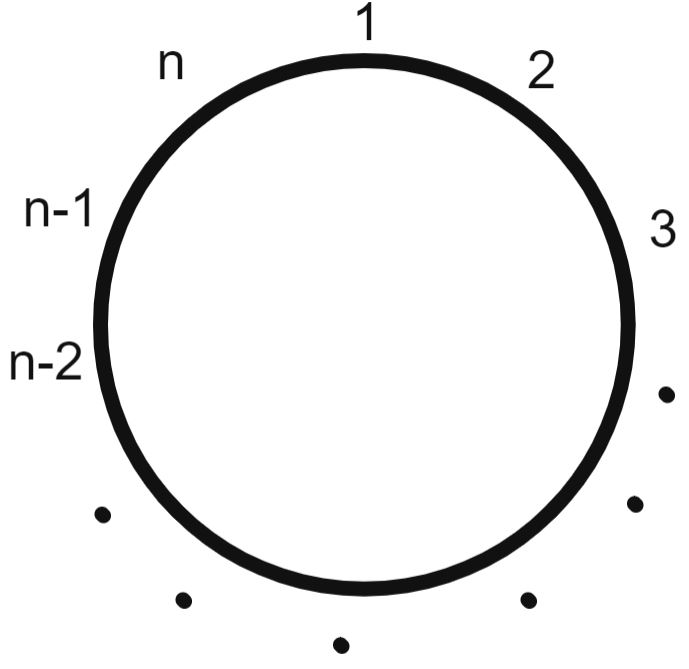
\includegraphics[width=\linewidth]{sol3} %тут поменять имя пикчи
    \end{figure}
    \end{minipage}
\end{minipage}

\textbf{Дефолтные математические знаки и символы:}\\
$\geqslant$,
$\leqslant$,
$a^{b}$,
$x_{i}$,
$\sqrt{a}$,
$\frac{a}{b}$,
$\displaystyle \frac{a}{b}$,
$\cdot$
$\;\Rightarrow\;$,
$\;\Leftrightarrow\;$,
$1{,}2$.
О промежутках:
$a\!b$,
$a\,b$,
$a\:b$,
$a\;b$,
$a\quad b$.

\textbf{Стандартные система и совокупность уравнений / неравенств:}\\
$\left\{
\begin{aligned}
f(x) &= 0 \\
g(x) &= 1
\end{aligned}\right.$

$\left[\begin{aligned}
&\left\{\begin{aligned}
f(x) &\geqslant a \\
g(x) &= b
\end{aligned}\right.\\
&\left\{\begin{aligned}
f(x) &< a \\
g(x) &= -b
\end{aligned}\right.
\end{aligned}\right.$

\subsection*{\textcolor{Emerald}{\textbf{Не математическое, но полезное:}}}
% комментарий в любом месте документа, который нигде не будет видно. Можно использовать для написания заметок-вопросов по задачам
\textbf{Пример таблицы:}

\begin{tabular}{|c|c|c|}
\hline
    $a$ & $b$ & текст
\\\hline
    $c$ & $d$ & мораль
\\\hline
\end{tabular}\\

\textbf{Отступы:} между\smallskip\\ строками\medskip\\ \textbf{Тире} --- это три дефиса.\\
\textbf{Списки:}
\begin{mylist}
\item [$\bullet$] это был пункт а
\item [2)] а это уже пункт номер 2 с изменённым заголовком
\end{mylist}

\subsection*{\textcolor{Emerald}{\textbf{Всё, неупомянутое выше (или если просто что-то не так):}}}
\begin{mylist}
\item [$\bullet$] Решение отдельных вопросов касательно ТеХа нужно искать в \href{https://www.mccme.ru/free-books/llang/newllang.pdf}{Львовском}.

\item [$\bullet$] Найти произвольный символ, который нужен, можно в \href{http://detexify.kirelabs.org/classify.html}{Detexify}.

\item [$\bullet$] Если возникли сомнения при решении, ответ практически ко всем задачам можно проверить с помощью \href{https://www.wolframalpha.com/}{WolframAlpha}.

\item [$\bullet$] Если в задаче нужно создать картинку, то лучше пока отложить эту задачу. Все графики планируется централизованно нарисовать (или перерисовать) в геогебре.

\item [\textcolor{brown}{\textbf{!!}}] Важно ставить \textcolor{red}{\textbf{$\spadesuit$}}
(или просто red) в тело задачи в случае серьёзных вопросов к решению и какой-то вопиющей лажи.

\item [\textcolor{brown}{\textbf{!!}}] Важно ставить \textcolor{olive}{\textbf{$\spadesuit$}}
(или просто olive) в тело задачи в случае не самого удачного текста и кривых отступов.
\end{mylist}

\subsection*{\textcolor{Violet}{\textbf{Комментарии:}}}% а также невидимые комментарии - так можно оставлять заметки-вопросы прямо в задаче, чтобы потом было понятно, в чём вопрос.
\begin{mylist}
\item [$\skull$] Переставлять задачи местами --- очень плохая идея.

\item [$\smiley$] При двойном клике по тексту pdf справа происходит автоматический переход к этому месту в латех-коде, а для обратного перехода можно нажать стрелку вправо (висит сверху между pdf и латех-кодом).

\item [$\smiley$] Если есть размышления, дописывать red/olive к задаче или не дописывать, то лучше всё-таки дописать.

\item [$\skull$] Самое плохое, что можно сделать --- написать в любое поле из трёх (НаписанноеРешение/ВерныйОтвет/Подсказка) только половину того, что надо, никак это не отметить, и потом пойти дальше.\\ Нужно в этот момент писать red/olive в случайном месте задачи, чтобы потом вычислить это с помощью Ctrl+F по всему документу (и это то, что потом будет делаться долго и тщательно)
\end{mylist}

\newpage
\setcounter{num}{256}

\hypertarget{6.6}{{\centering\section*{\bigskip\\\textcolor{Blue}{\hyperlink{start2}{\textcolor{Blue}{6.6}} Координатная прямая и модуль числа.}\vspace{-5mm}}}}

\begin{problem}{Координаты на прямой.}{6.6.1}{6S}{(лёгкая)}
{Некоторые величины можно понимать в двух противоположных смыслах: например, 5 градусов тепла --- 5 градусов холода, 1000 рублей выигрыш --- 1000 рублей проигрыш. Придумай хотя бы ещё 2 примера таких величин.}
{НаписанноеРешение}
{Расстояние, прибыль, высота над уровнем моря, время UTC+/UTC-}{Подсказка}
\end{problem}

\begin{problem}{Координаты на прямой.}{6.6.1}{6S}{(лёгкая)}
{Расставь точки на координатной прямой в правильном порядке и угадай зашифрованное слово: $\;A (0{,}21);\; C (2{,}001);\; E(10{,}2);\; R(-0{,}012);\; N(1{,}2);\; F(-0{,}201)$.}
{Точки $R$ и $F$ --- единственные, которые имеют отрицательную координату. Поэтому они находятся левее всех, и так как $-0{,}201 < -0{,}012$, точка $F$ находится левее $R$. Теперь оставшиеся точки $A$, $C$, $E$, $N$: $0{,}21 < 1{,}2 < 2{,}001 < 10{,}2$. То есть эти 4 точки расположены в таком порядке: $A - N - C - E$.
\vspace{-4mm}\\\begin{minipage}{\linewidth}
    \begin{minipage}{0.45\linewidth}
    ~\vspace{2mm}\\
    Смотрим, что получилось:
    \end{minipage}
    \hspace{0.02\linewidth}
    \begin{minipage}{0.5\linewidth}\begin{figure}[H] 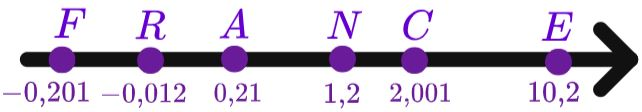
\includegraphics[width=\linewidth]{sol76}\end{figure}\end{minipage}
\end{minipage}}
{Точки расположены в следующем порядке: $F - R - A - N - C - E$.\\ То есть зашифрованное слово --- France (Франция).}{Расположи точки в порядке возрастания!}
\end{problem}

\begin{problem}{Координаты на прямой.}{6.6.1}{6K}{*}
{Нарисуй на координатной прямой точки $\displaystyle A \left(\frac{10}{59}\right)$, $\displaystyle B \left(\frac{2}{15}\right)$, $\displaystyle C \left(\frac{1}{6}\right)$ и $\displaystyle D \left(\frac{10}{61}\right)$ в порядке возрастания.}
{Для того, чтобы расставить числа в порядке возрастания, сравним их друг с другом: для этого проще всего сравнивать дроби с одинаковыми числителями: $\frac{2}{15} = \frac{10}{75}$, $\frac16 = \frac{10}{60}$. Как мы знаем, из двух дробей с равными числителями больше та, знаменатель которой меньше. Поэтому получаем, что $\frac{10}{75} < \frac{10}{61} < \frac{10}{60} < \frac{10}{59}$.
\vspace{-4mm}\\\begin{minipage}{\linewidth}
    \begin{minipage}{0.59\linewidth}
    ~\vspace{2mm}\\
    То есть $\frac{2}{15} < \frac{10}{61} < \frac16 < \frac{10}{59}$, и порядок точек на прямой будет таким, как на рисунке справа:\\ $B$, потом $D$, потом $C$, и правее всех --- $A$.
    \end{minipage}
    \hspace{0.02\linewidth}
    \begin{minipage}{0.38\linewidth}\begin{figure}[H] 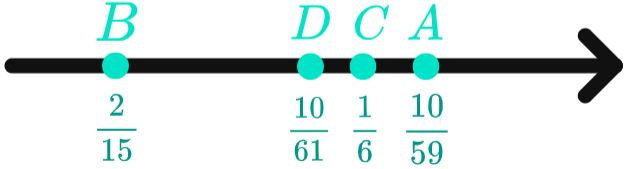
\includegraphics[width=\linewidth]{sol75}\end{figure}\end{minipage}
\end{minipage}}
{$B - D - C - A$. Смотри рисунок выше.}{Сравни все эти дроби. Рисунок можно нарисовать приближённо.}
\end{problem}

\begin{problem}{Координаты на прямой.}{6.6.1}{6K}{(лёгкая)}
{Точки $A$, $B$, и $C$ расположены на координатной прямой. Координата точки $A$ равна $17$, координата точки $C$ равна $-7$. Точка $B$ находится ровно посередине между $A$ и $C$. Какова её координата?}
{НаписанноеРешение}
{ВерныйОтвет}{Подсказка}
\end{problem}

\begin{problem}{Координаты на прямой.}{6.6.1}{6K}{(лёгкая)}
{Точки $A$, $B$, и $C$ расположены на координатной прямой. Координата точки $A$ равна $4$, длина отрезка $AB$ равна $7$, длина отрезка $BC$ равна $5$.\\ Какова координата точки $C$, если известно, что она отрицательна?}
{Длина отрезка $AB$ равна 7. Это означает, что точка $B$ находится либо на 7 левее точки $A$, либо на 7 правее. В первом случае её координата будет равна $4 - 7 = -3$, а во втором случае $4 + 7 = 11$. Поскольку нам известно, что длина отрезка $BC$ равна 5, и координата точки $C$ отрицательна, координата точки $B$ никак не может быть равна 11. Значит, координата точки $B$ равна $-3$.\\ Тогда, если точка $C$ находится левее точки $B$ на координатной прямой, её координата будет равна $-3 - 5 = -8$, а если правее, то $-3 + 5 = 2$.\\ Во втором случае координата $C$ не отрицательна, то есть этот вариант нам не подходит. Остался единственный вариант --- и координата точки $C$ равна $-8$.}
{Координата точки $C$ равна $-8$.}{Точка $B$ находится или левее точки $A$, или правее.\\ Какой вариант из этих двух нам подходит, а какой --- нет?}
\end{problem}

\begin{problem}{Координаты на прямой.}{6.6.1}{6K}{(лёгкая)}
{Точки $A$, $E$, и $I$ расположены на координатной прямой.\\ Координата точки $A$ равна $7$, координата точки $E$ равна $-5$.\\ Точка $I$ расположена так, что $AI$ составляет ровно $\frac{2}{3}$ от длины отрезка $AE$.\\ Какова координата точки $I$, если известно, что она положительна?}
{НаписанноеРешение}
{ВерныйОтвет}{Подсказка}
\end{problem}

\begin{problem}{Координаты на прямой.}{6.6.1}{6K}{(лёгкая)}
{Точки $A$, $B$, и $C$ расположены на координатной прямой. Координата точки $A$ равна $7$, точка $B$ имеет координату $-2$. Точка $C$ такова, что её координата положительна, а длина отрезка $AB$ составляет треть от длины отрезка $BC$.\\ Какова координата точки $C$?}
{Длина отрезка $AB$ составляет $7 - (-2) = 7 + 2 = 9$. Нам известно, что длина отрезка $AB$ составляет треть от длины отрезка $BC$, что означает, что длина отрезка $BC$ втрое больше и равна $9\cdot 3 = 27$. Координата точки $C$ тогда равна $-2 \pm 27$, то есть или $-2 - 27 = -29$, или $-2 + 27 = 25$. Так как координата точки $C$ должна быть положительна, получаем, что её координата равна $25$.}
{Координата точки $C$ равна 25.}{Чему равна длина отрезка $AB$? Отрезка $BC$?\\ Находится точка $C$ левее или правее точки $B$?}
\end{problem}

\begin{problem}{Координаты на прямой.}{6.6.1}{6K}{*}
{Точки $A_1$, $A_2$, $\ldots$, $A_7$, $A_8$ расположены на координатной прямой. Координата точки $A_1$ равна $0$, расстояние от первой точки до второй равно $1$, от второй до третьей равно $2$, $\ldots$ , расстояние от седьмой до восьмой точки равно $7$.\\ Точка $A_8$ расположена так, что середина отрезка $A_1 A_8$ расположена так близко к нулю, как это только возможно. Чему равна координата точки $A_8$?}
{Эту задачу можно решить полным перебором, однако приведу чуть более изящное решение. Поскольку координата точки $A_1$ равна 0, а длина отрезка $A_1A_2$ равна 1, то координата точки $A_2$ равна или $+1$, или $-1$.\\ Далее, поскольку длина отрезка $A_2A_3$ равна 2, то к координате или прибавится 2, если точка $A_3$ правее точки $A_2$, или из неё вычтется 2, если левее.\\ И так далее для каждой точки --- или прибавляем, или отнимаем. Поэтому в итоге мы получим координату точки $A_8$, равную $0 \pm 1 \pm 2 \pm 3 \pm 4 \pm 5 \pm 6 \pm 7$ (на месте каждого знака $\pm$ должен стоять или плюс, или минус).\\
Чтобы середина отрезка $A_1A_8$ была ближе к нулю, $A_8$ должно быть ближе к нулю. Оказывается, можно сделать так, чтобы координата $A_8$ была равна нулю!\\ То есть надо расставить знаки <<$+$>> и <<$-$>> в арифметическом примере (см. ниже)
$$0 \phantom{+} 1 \phantom{+} 2 \phantom{+} 3 \phantom{+} 4 \phantom{+} 5 \phantom{+} 6 \phantom{+} 7 = 0.$$
У этого примера есть множество решений, например, три приведённые ниже:
$$0 + 1 + 2 - 3 + 4 - 5 - 6 + 7 = 0.$$
$$0 - 1 + 2 + 3 + 4 + 5 - 6 - 7 = 0.$$
$$0 + 1 - 2 + 3 + 4 - 5 + 6 - 7 = 0.$$
Получающиеся точки на координатной прямой в каждом из этих трёх случаев:
\vspace{-4mm}\\\begin{minipage}{\linewidth}
    \begin{figure}[H]
    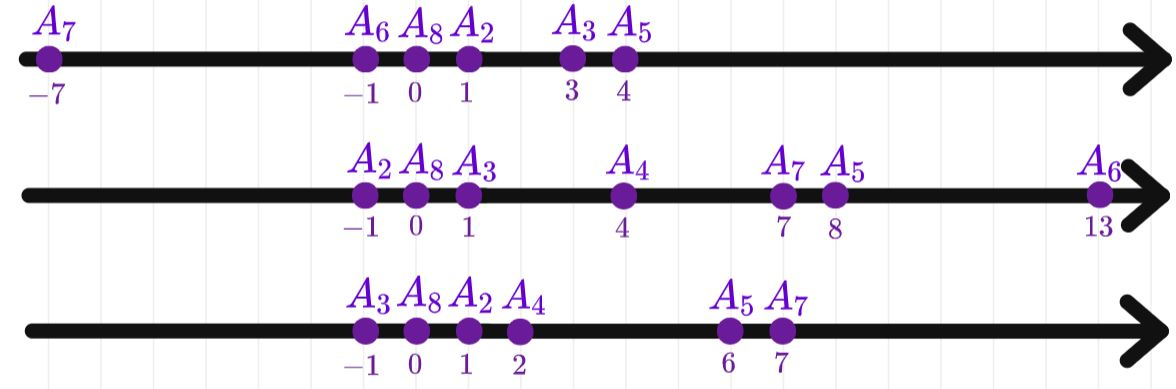
\includegraphics[width=\linewidth]{sol78}
    \end{figure}
\end{minipage}}
{Координата точки $A_8$ в этом случае равна 0.}{Надо понять, почему самый лучший вариант --- когда координата точки $A_8$ равна 0, а затем показать, как этот случай можно получить.}
\end{problem}

\begin{problem}{Координаты на прямой.}{6.6.1}{6K}{*}
{Точки $A$, $B$, и $C$ расположены на прямой, $D$~--- середина отрезка $AB$. Отрезок $AB$ равен трём отрезкам $AC$, длина отрезка $CD$ вдвое меньше длины отрезка $AC$.\\ Во сколько раз отрезок $BC$ больше отрезка $CD$?}
{Изобразим на рисунке то, что нам уже известно, чтобы было, от чего отталкиваться. Мы знаем, что $D$ делит отрезок $AB$ пополам. Также, поскольку отрезок $AB$ в три раза больше, чем $AC$, отрезок $AC$ втрое меньше, чем $AB$. \vspace{-4mm}\\\begin{minipage}{\linewidth}
    \begin{minipage}{0.47\linewidth}
    ~\vspace{1mm}\\
    В результате получается картина, изображённая на рисунке справа:
    \end{minipage}
    \hspace{0.02\linewidth}
    \begin{minipage}{0.5\linewidth}\begin{figure}[H] 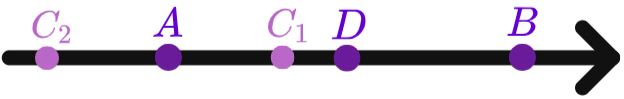
\includegraphics[width=\linewidth]{sol77}\end{figure}\end{minipage}
\end{minipage}
Точка $C$ может находиться в одном из двух отмеченных мест --- либо в точке $C_1$, либо в точке $C_2$ (и $AC_1$, и $AC_2$ втрое меньше $AB$). Теперь осталось использовать последнее условие: отрезок $CD$ должен быть вдвое меньше отрезка $AC$.\\ Становится очевидно, что $C$ не может находиться в точке $C_2$, поскольку в этом случае отрезок $CD$ наоборот, больше отрезка $AC$. Значит, $C_1$ --- это и есть $C$.\smallskip\\
Проверка: длина $AD$ составляет половину $AB$, длина $AC_1$ равна $\frac13 AB$, поэтому длина отрезка $CD$ равна $\frac12 AB - \frac13 AB = \frac16 AB$, что вдвое меньше отрезка $AC$.\smallskip\\ Длина отрезка $BC$ же равна сумме длин отрезков $BD$ и $CD$, то есть $\frac12 AB + \frac16 AB = \frac23 AB$. Получается, что отрезок $BC$ составляет $\frac23 AB = \frac46 AB$, а отрезок $CD$ --- $\frac16 AB$. Поэтому отрезок $BC$ больше отрезка $CD$ в 4 раза.}
{Отрезок $BC$ больше отрезка $CD$ в 4 раза.}{Нарисуй точки $A$, $B$, $D$.\\ Где может находиться точка $C$ c учётом обоих условий?}
\end{problem}

\begin{problem}{Противоположные числа.}{6.6.2}{Киселев}{(лёгкая)}
{Когда скорый поезд был на расстоянии 100 км от станции Бологое (эта станция находится приблизительно посередине между Москвой и Санкт-Петербургом), почтовый поезд едущий в противоположную сторону, был на расстоянии 50 км от Бологого. На каком расстоянии находились тогда эти два поезда друг от друга?\\ Правда ли, что есть два возможных ответа?}
{НаписанноеРешение}
{ВерныйОтвет}{Подсказка}
\end{problem}

\begin{problem}{Модуль числа.}{6.6.3}{6K}{*}
{Точки $A$, $B$, $C$, и $D$ расположены на прямой. Координата точки $A$ равна $0$, длина отрезка $AB$ равна $3$, длина отрезка $BC$ равна $2$, отрезка $CD$~--- $5$.\\ Чему равен модуль координаты точки $C$, если длина отрезка $AD$ равна $4$?}
{НаписанноеРешение}
{ВерныйОтвет}{Подсказка}
\end{problem}

\begin{problem}{Сравнение чисел.}{6.6.4}{6K}{(лёгкая)}
{Сравнить числа $\,1{,}35\,$ и $\,\displaystyle\frac{27}{25}$.}
{НаписанноеРешение}
{ВерныйОтвет}{Подсказка}
\end{problem}

\begin{problem}{Сравнение чисел.}{6.6.4}{6K}{(лёгкая)}
{Что больше, 1/7 или $0{,}1428$?}
{Для сравнения двух дробей, $\frac17 \,\vee\, \frac{1428}{10000}$ приведём их к одному числителю: $\frac17 = \frac{1428}{7\cdot1428} = \frac{1428}{9800 + 140 + 56} = \frac{1428}{9996}$. То есть нам нужно сравнить $\frac{1428}{9996} \,\vee\, \frac{1428}{10000}$. Числители этих двух дробей равны, значит больше будет та, знаменатель которой меньше. Поэтому $\frac17 > 0{,}1428$.}
{$\frac17$ больше, чем $0{,}1428$.\\
Её можно представить в виде бесконечной десятичной дроби: $\frac17 = 0{,}(142857)$.}{Для сравнения двух дробей следует сравнивать или две десятичные дроби, или две обыкновенные по одному из правил сравнения.}
\end{problem}

\begin{problem}{Сравнение чисел.}{6.6.4}{6K}{(лёгкая)}
{Иван ездит на метро. Одна поездка по Тройке стоит $38$ рублей, а безлимитный билет на месяц~--- $1900$ рублей. Сколько поездок в месяц нужно делать, чтобы покупка безлимитного билета имела смысл?}
{НаписанноеРешение}
{ВерныйОтвет}{Подсказка}
\end{problem}

\begin{problem}{Сравнение чисел.}{6.6.4}{6K}{(лёгкая)}
{Что выгоднее с экономической точки зрения, покупать развесной творог стоимостью $360$ рублей/килограмм или творог в пачках по $180$ грамм, стоимостью $66$ рублей каждая? Сколько будет стоить $900$ грамм творога в этом случае?}
{НаписанноеРешение}
{ВерныйОтвет}{Подсказка}
\end{problem}

\begin{problem}{Сравнение чисел.}{6.6.4}{6K}{(лёгкая)}
{Петя очень редко ездит на автобусе. Он школьник и может купить льготный билет без ограничения числа поездок за $265$ рублей. Если его не покупать, одна поездка будет стоить $40$ рублей. Сколько поездок в месяц может делать Петя, если ему выгоднее купить льготный билет, но он бывает в автобусе меньше $10$ раз в месяц?

}
{Если бы Петя не покупал льготный билет и делал за месяц $k$ поездок, он бы тратил $40 \cdot k$ рублей. Но поскольку ему выгоднее купить льготный билет, это значит, что 265 рублей меньше, чем $40k$, то есть $265 < 40k$. При $k = 6$ он бы тратил $40 \cdot 6 = 240$ рублей, а при $k = 7$ --- $40 \cdot 7 = 280$ рублей. Значит, $k \geqslant 7$, так как сумма должна быть больше 265 рублей (чтобы было выгоднее сэкономить).\\
Нам известно, что Петя бывает в автобусе меньше 10 раз в месяц. Значит, за месяц он делает 7, 8, или 9 поездок на автобусе --- точнее мы сказать не можем.}
{Петя делает семь, восемь, или девять поездок на автобусе за месяц.}{Сколько бы Петя заплатил за все поездки на автобусе, если бы он не купил льготный билет? Почему он его всё-таки купил? Ответов несколько.}
\end{problem}

\begin{problem}{Сравнение чисел.}{6.6.4}{6K}{(лёгкая)}
{Телефонная компания предлагает абоненту два тарифа на выбор: поминутный (оплата $0{,}65$ рублей за минуту) и безлимитный (оплата 500 рублей в месяц). Сколько заплатит абонент, если за месяц он потратит 700 минут, и выберет самый выгодный для себя тариф?}
{Если использовать поминутный тариф, за 700 минут придётся заплатить $700 \cdot 0{,}65 = 7 \cdot 65 = 455$ р. Если же использовать безлимитный тариф, оплата составит 500 р. Следовательно, выбирать надо поминутный тариф.}
{Абонент заплатит всего 455 р, если выберет поминутный тариф.}{Сколько придётся заплатить, если выбрать поминутный тариф?}
\end{problem}

\begin{problem}{Сравнение чисел.}{6.6.4}{6K}{(лёгкая)}
{В ближайшем магазине 1 кг гречки стоит 96 рублей. В более далёком магазине 1 кг гречки стоит 90 рублей, но проезд туда и обратно стоит 50 рублей.\\ За каким наименьшим целым количеством килограммов гречки имеет смысл ездить в более далёкий магазин?}
{НаписанноеРешение}
{ВерныйОтвет}{Подсказка}
\end{problem}

\begin{problem}{Сравнение чисел.}{6.6.4}{6K}{(лёгкая)}
{Алексей заказывает себе на дачу батут и думает, в какой компании оформлять доставку. В компании <<Всем привезём>> доставка стоит $500$ рублей, но за каждый километр от МКАД нужно доплачивать по $30$ рублей. В компании <<Привезём быстро>> доставка стоит $400$ рублей, а за каждый километр от МКАД нужно доплачивать по $40$ рублей. Где надо заказывать батут и во сколько обойдётся доставка, если дача находится в $16$ километрах от МКАД?}
{Рассмотрим оба варианта. Если заказывать доставку в компании <<Всем привезём>>, то общая сумма доставки составит $500 + 30\cdot16 = 500 + 480 = 980$ р.\\ Если же выбрать компанию <<Привезём быстро>>, вся доставка обойдётся в $400 + 40\cdot16 = 400 + 640 = 1040$ рублей. Следовательно, <<Всем привезём>> выгоднее.}
{Батут надо заказывать в компании <<Всем привезём>>, сумма доставки составит 980 р.}{Сколько придётся заплатить в каждом случае?}
\end{problem}

\begin{problem}{Сравнение чисел.}{6.6.4}{7A}{(лёгкая)}
{От Академической до Баррикадной можно доехать за 8 остановок с одной пересадкой или за 6 остановок с двумя пересадками. Какой вариант быстрее и на сколько секунд, если поезд проезжает одну остановку за 145 секунд, а на пересадку уходит примерно 3 минуты? Сколько времени это займёт?}
{3 минуты --- это $3 \cdot 60 = 180$ секунд. Это значит, что на первый вариант с 8 остановками и одной пересадкой уходит $8\cdot 145 + 180 = 1160 + 180 = 1340$ секунд, а на второй вариант --- $6 \cdot 145 + 2 \cdot 180 = 870 + 360 = 1230$ секунд. Поэтому вариант с двумя пересадками быстрее по времени, маршрут займёт $1230 : 60 = 20{,}5$ минут.}
{Быстрее ехать с двумя пересадками, на дорогу уйдёт $20{,}5$ минут.}{Проще всего посчитать время в секундах.}
\end{problem}

\begin{problem}{Сравнение чисел.}{6.6.4}{6K}{(лёгкая)}
{Как всем известно, бобры добры и знают секрет крепких зубов. Для этого они чистят зубы пастой по $5$ раз в день. Сами они пасту купить не могут, поэтому снимаются в рекламе, за которую им дают $100$ пачек пасты.\\ Для взрослого бобра пачки хватает на $3$ дня, для маленького~--- на $5$.\\ На плотине живёт $10$ взрослых бобров и $15$ маленьких бобрят.\\ Сколько раз в месяц ($30$ дней) им надо сниматься в рекламе?}
{НаписанноеРешение}
{ВерныйОтвет}{Подсказка}
\end{problem}

\begin{problem}{Сравнение чисел.}{6.6.4}{9I}{*}
{После каждой стирки кусок мыла уменьшается на 20\%.\\ После скольких стирок он уменьшится больше, чем на треть?}
{НаписанноеРешение}
{ВерныйОтвет}{Подсказка}
\end{problem}

\end{document}